% Bab III  Metode Penelitian
\chapter{METODE PENELITIAN}

\section{Lokasi dan Waktu Penelitian}
Sebutkan lokasi penelitian dengan jelas dan lengkap, serta lama atau masa pengumpulan data.

\section{Alat dan Bahan}
Sebutkan nama, spesifikasi, dan produsen peralatan serta bahan penelitian. Daftar alat dan bahan dapat disajikan dalam tabel, seperti Tabel 3.1 (nama, spesifikasi, dan jumlah pada tabel adalah contoh).

\begin{singlespace}
\begin{longtable}{|c|p{0.26\linewidth}|p{0.30\linewidth}|c|}
\caption{Contoh daftar alat dan bahan penelitian}\\
\hline
\textbf{No.} & \textbf{Nama} & \textbf{Spesifikasi} & \textbf{Jumlah} \\
\hline
1 & Papan ESP32 & Dua inti 240 MHz, Wi-Fi 2,4 GHz & 1 \\
\hline
2 & Sensor DHT22 & Suhu $-40$ sampai 80 $^\circ$C, galat $\pm$0,5 $^\circ$C & 3 \\
\hline
3 & Modul relay & 5 V, satu kanal & 1 \\
\hline
4 & Layar LCD 16$\times$2 & Antarmuka I2C & 1 \\
\hline
5 & Laptop & Prosesor 4 inti, RAM 8 GB & 1 \\
\hline
\end{longtable}
\end{singlespace}

\textit{Contoh kalimat bersitasi:} Prosedur pengujian mengacu pada penelitian sebelumnya (AlQahtani \& Alhassany, 2013).

\section{Tahapan Penelitian}
Jelaskan tahapan penelitian secara berurutan sehingga orang lain dapat mengulangi penelitian dengan cara yang sama. Tahapan dapat digambarkan dengan diagram alir (\textit{flowchart}) menggunakan simbol standar, seperti Gambar 3.1 (isi diagram adalah contoh).

\begin{figure}[H]
\centering
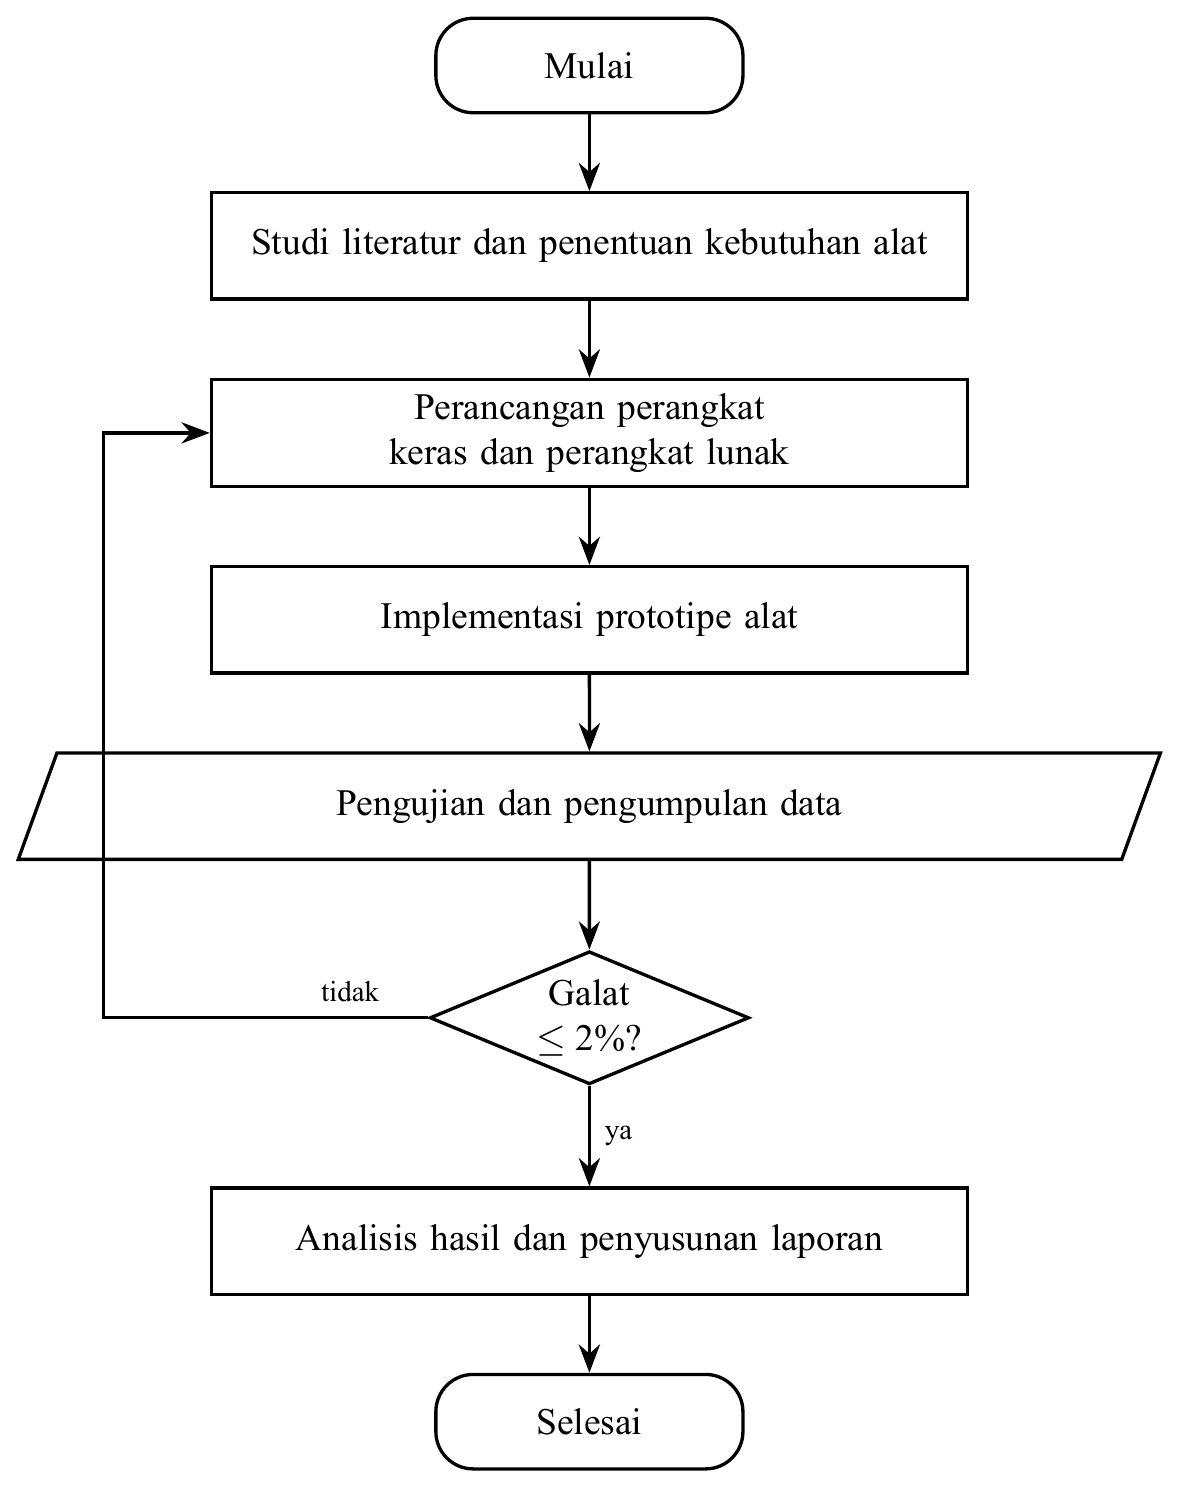
\includegraphics[width=0.5\textwidth]{../00-gambar/contoh-alur.png}
\caption{Contoh diagram alir tahapan penelitian}
\end{figure}

\section{Perancangan Sistem}
Uraikan rancangan sistem yang digunakan beserta cara penerapannya. Rancangan perangkat keras dapat ditunjukkan dengan skema rangkaian, seperti Gambar 3.2 (nama pin pada gambar adalah contoh).

\begin{figure}[H]
\centering
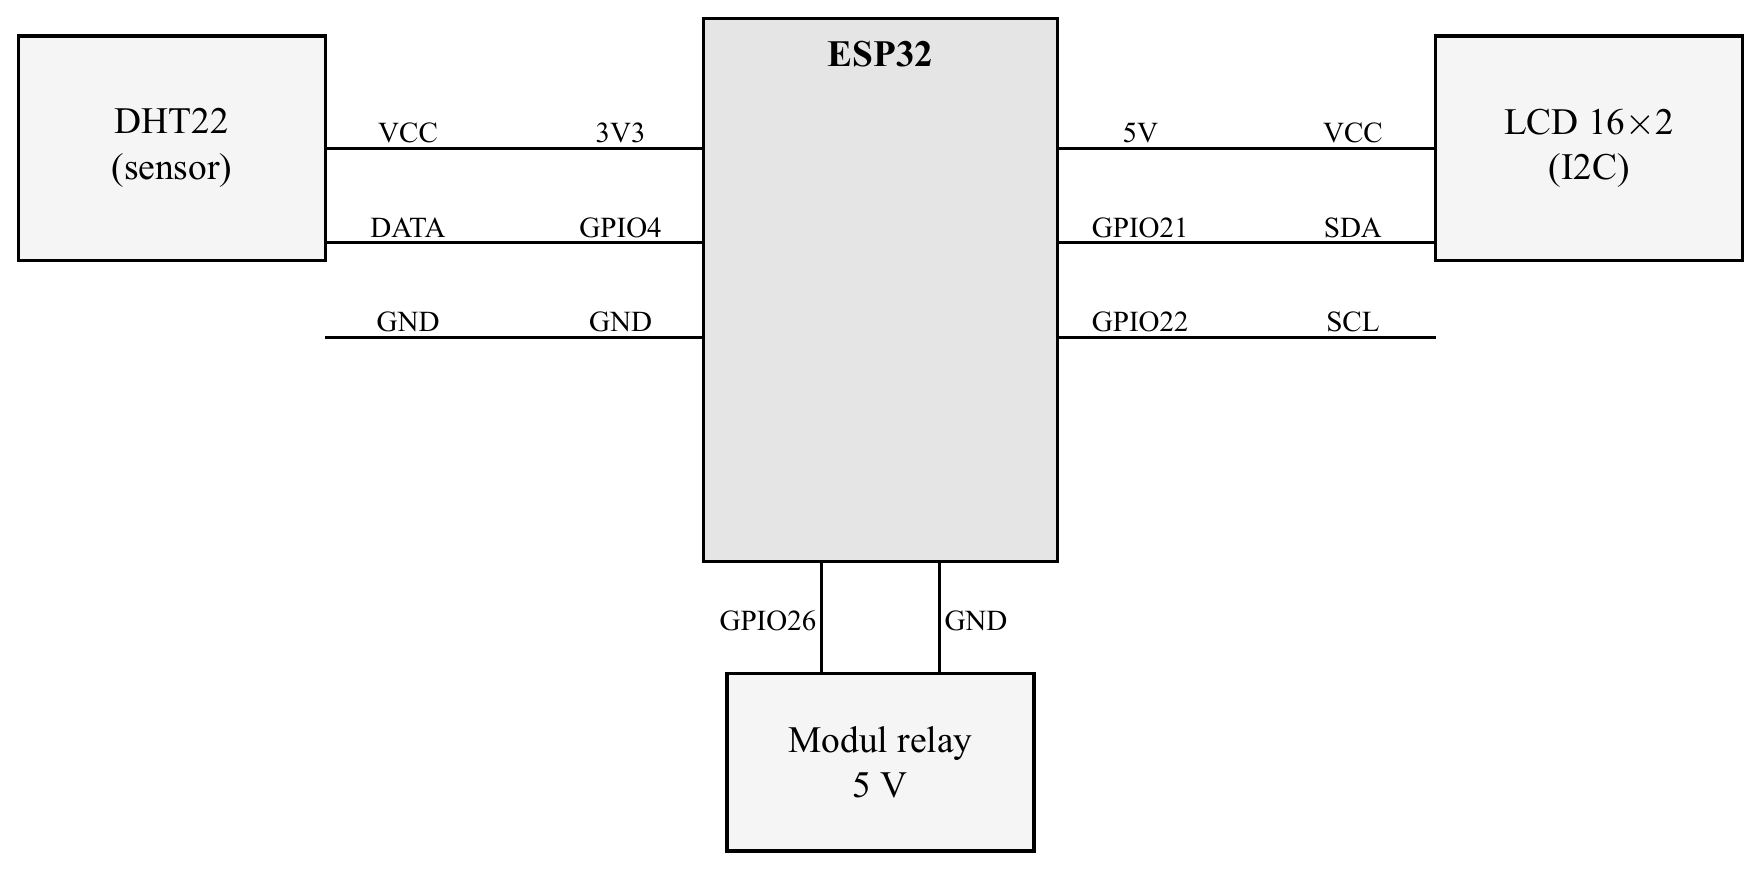
\includegraphics[width=0.95\textwidth]{../00-gambar/contoh-rangkaian.png}
\caption{Contoh skema rangkaian perangkat keras}
\end{figure}

\section{Variabel Pengamatan dan Analisis Data}
Sebutkan variabel bebas dan variabel terikat yang diamati, serta teknik pengumpulan dan analisis data yang digunakan.
